\documentclass[10pt,twoside]{article}
\usepackage[paperwidth=6in,paperheight=9in,top=0.82in,bottom=0.78in,inner=0.84in,outer=0.68in,headsep=17pt,footskip=28pt]{geometry}
\usepackage{fontspec}
\IfFontExistsTF{Tiempos Text}{\setmainfont{Tiempos Text}}{\setmainfont{TeX Gyre Pagella}}
\IfFontExistsTF{Söhne}{\setsansfont{Söhne}}{\setsansfont{Latin Modern Sans}}
\usepackage{xcolor}
\definecolor{NaturalPaper}{HTML}{FAF8F3}
\definecolor{Carbon}{HTML}{202124}
\definecolor{WarmGrey}{HTML}{6C6A66}
\definecolor{StoneRule}{HTML}{B7B0A6}
\definecolor{QuietUmber}{HTML}{7B4B3A}
\definecolor{NotePaper}{HTML}{F2EEE8}
\pagecolor{NaturalPaper}
\color{Carbon}
\usepackage{graphicx}
\usepackage{tikz}
\usepackage{microtype}
\usepackage{setspace}
\usepackage{tcolorbox}
\tcbuselibrary{breakable,skins}
\usepackage{fancyhdr}
\usepackage{titlesec}
\usepackage{hyperref}
\usepackage{etoolbox}
\hypersetup{colorlinks=true,linkcolor=Carbon,urlcolor=Carbon,citecolor=Carbon,pdftitle={The Age of Operational AI — Editorial Specimen v2},pdfauthor={Steve BA-NDOUWE}}
\setlength{\parindent}{4.5mm}
\setlength{\parskip}{0pt}
\linespread{1.18}\selectfont
\emergencystretch=1.2em
\frenchspacing
\titleformat{\section}{\sffamily\bfseries\large\color{Carbon}}{\thesection}{0.65em}{}
\titlespacing*{\section}{0pt}{18pt}{7pt}
\titleformat{\subsection}{\sffamily\bfseries\normalsize\color{Carbon}}{}{0pt}{}
\titlespacing*{\subsection}{0pt}{15pt}{5pt}
\renewcommand{\thesection}{\arabic{section}}
\setcounter{secnumdepth}{-1}
\setcounter{tocdepth}{1}
\newcommand{\CurrentRunningHead}{}
\newtcolorbox{evidencebox}[1][]{enhanced,breakable,colback=NotePaper,colframe=NotePaper,boxrule=0pt,left=11pt,right=11pt,top=8pt,bottom=8pt,borderline west={1.3pt}{0pt}{QuietUmber},fonttitle=\sffamily\bfseries\footnotesize\color{QuietUmber},title={#1},coltitle=QuietUmber}
\renewenvironment{quote}{\begin{evidencebox}}{\end{evidencebox}}
\pagestyle{fancy}
\fancyhf{}
\fancyhead[LE]{\sffamily\fontsize{7}{8}\selectfont\color{WarmGrey}THE AGE OF OPERATIONAL AI}
\fancyhead[RO]{\sffamily\fontsize{7}{8}\selectfont\color{WarmGrey}\CurrentRunningHead}
\fancyfoot[LE,RO]{\sffamily\fontsize{7}{8}\selectfont\color{WarmGrey}\thepage}
\renewcommand{\headrulewidth}{0.25pt}
\renewcommand{\headrule}{\hbox to\headwidth{\color{StoneRule}\leaders\hrule height \headrulewidth\hfill}}
\newcommand{\coverpage}{%
\clearpage\thispagestyle{empty}%
\begin{tikzpicture}[remember picture,overlay]
\node[anchor=center,inner sep=0pt] at (current page.center) {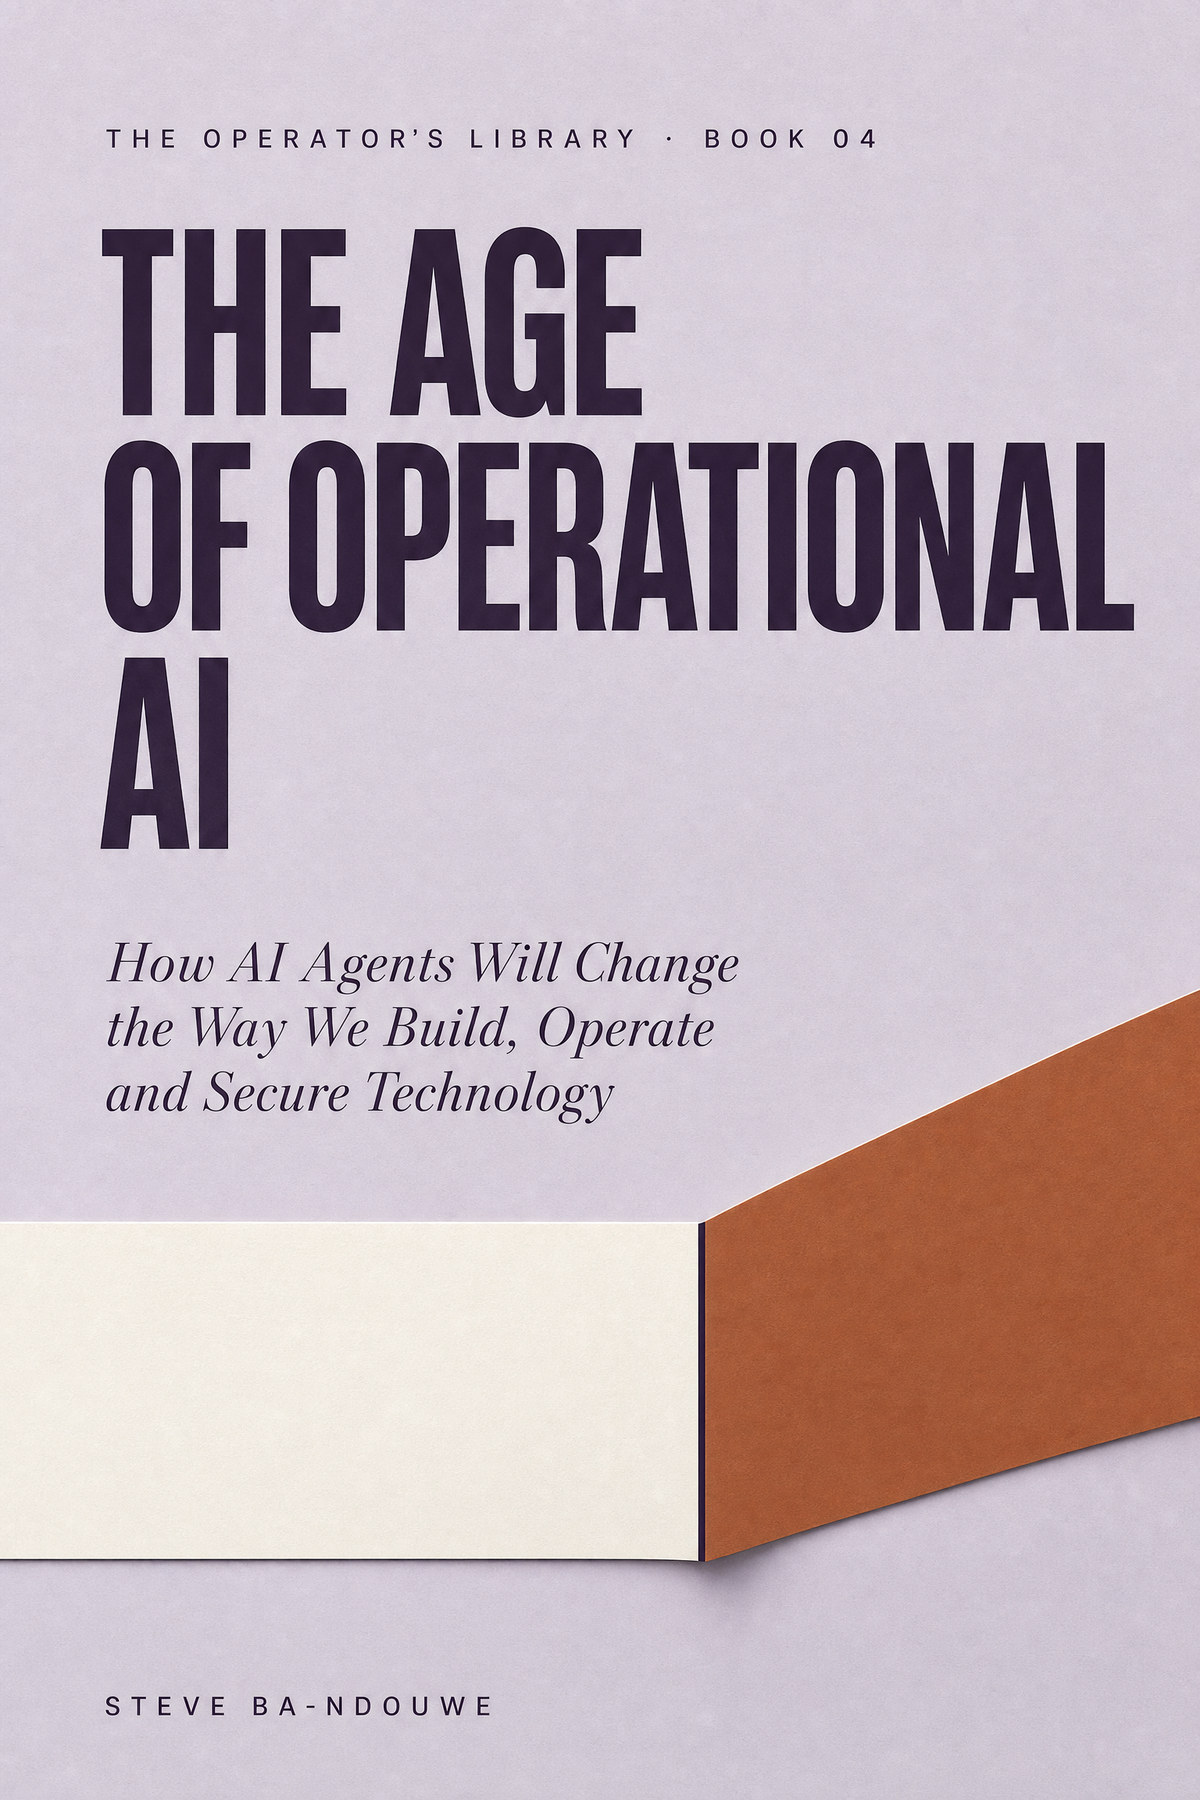
\includegraphics[width=\paperwidth,height=\paperheight]{../assets/book4-front-cover-print-light.jpg}};
\end{tikzpicture}\mbox{}\clearpage}
\newcommand{\halfTitle}{%
\clearpage\thispagestyle{empty}\vspace*{0.35\textheight}
{\sffamily\fontsize{24}{28}\selectfont\bfseries THE AGE OF\\ OPERATIONAL AI}\par\vfill
{\sffamily\fontsize{7}{9}\selectfont\color{WarmGrey}THE OPERATOR'S LIBRARY · BOOK 04}\clearpage}
\newcommand{\titlePage}{%
\clearpage\thispagestyle{empty}\vspace*{0.23\textheight}
{\sffamily\fontsize{8}{10}\selectfont\color{QuietUmber}THE OPERATOR'S LIBRARY · BOOK 04}\par\vspace{19pt}
{\sffamily\fontsize{29}{33}\selectfont\bfseries THE AGE OF\\ OPERATIONAL AI}\par\vspace{16pt}
{\itshape\large How AI Agents Will Change the Way\\ We Build, Operate and Secure Technology}\par\vfill
{\sffamily\fontsize{9}{11}\selectfont STEVE BA-NDOUWE}\clearpage}
\newcommand{\copyrightPage}{%
\clearpage\thispagestyle{empty}\vspace*{0.65\textheight}
{\footnotesize © 2026 Steve BA-NDOUWE. All rights reserved.\\
First editorial specimen, prepared for design and reading review.\\
The final edition will include verified source notes and publication data.}\clearpage}
\newcommand{\introductionOpener}{%
\phantomsection\addcontentsline{toc}{section}{Introduction: The Terms of Delegation}
\renewcommand{\CurrentRunningHead}{INTRODUCTION}
\clearpage\thispagestyle{empty}\vspace*{0.18\textheight}
{\sffamily\fontsize{8}{10}\selectfont\color{QuietUmber}INTRODUCTION}\par\vspace{18pt}
{\sffamily\fontsize{31}{35}\selectfont\bfseries THE TERMS OF\\ DELEGATION}\par\vspace{20pt}
{\itshape\large Before an organisation gives a system the right to act, it must decide what it is delegating, what it will retain, and how it will know the difference.}\par\vfill
{\sffamily\fontsize{7}{9}\selectfont\color{WarmGrey}THE OPERATOR'S LIBRARY}\clearpage}
\newcommand{\partOpener}{%
\phantomsection\addcontentsline{toc}{part}{Part I. The Shift}
\clearpage\thispagestyle{empty}\vspace*{0.18\textheight}
{\sffamily\fontsize{10}{12}\selectfont\color{QuietUmber}PART I}\par\vspace{18pt}
{\sffamily\fontsize{34}{38}\selectfont\bfseries THE SHIFT}\par\vspace{18pt}
{\itshape\large The transition from systems that follow instructions to systems that interpret objectives and act within them.}\par\vfill
{\sffamily\fontsize{7}{9}\selectfont\color{WarmGrey}WHAT CHANGES WHEN SOFTWARE HAS DISCRETION}\clearpage}
\newcommand{\chapterThreeOpener}{%
\phantomsection\addcontentsline{toc}{section}{3. The Operator Gets a Copilot}
\renewcommand{\CurrentRunningHead}{THE OPERATOR GETS A COPILOT}
\clearpage\thispagestyle{empty}\vspace*{0.18\textheight}
{\sffamily\fontsize{8}{10}\selectfont\color{QuietUmber}CHAPTER 3}\par\vspace{18pt}
{\sffamily\fontsize{30}{34}\selectfont\bfseries THE OPERATOR GETS\\ A COPILOT}\par\vspace{19pt}
{\itshape\large What changes when a system can prepare much of the work but must not own its result.}\par\vfill
{\sffamily\fontsize{7}{9}\selectfont\color{WarmGrey}PART I · THE SHIFT}\clearpage}
\newcommand{\chapterCoda}{%
\clearpage\thispagestyle{empty}\vspace*{0.22\textheight}
{\sffamily\fontsize{8}{10}\selectfont\color{QuietUmber}CHAPTER CODA}\par\vspace{18pt}
{\sffamily\fontsize{23}{28}\selectfont\bfseries WHAT REMAINS}\par\vspace{18pt}
{\large A copilot can prepare work.\\[7pt]
The operator still owns the evidence and the decision.\\[7pt]
The organisation must retain the boundary.}\par\vspace{30pt}
\noindent\rule{0.25\textwidth}{0.5pt}\par\vspace{12pt}
{\itshape\large Assistance becomes a different operational relationship when the system is permitted to carry its recommendation into action.}\par\vfill
{\sffamily\fontsize{7}{9}\selectfont\color{WarmGrey}NEXT · THE MOMENT A HELPFUL SYSTEM BEGINS TO ACT}\clearpage}
\newcommand{\sourceNotesOpener}{%
\clearpage\thispagestyle{empty}\vspace*{0.2\textheight}
{\sffamily\fontsize{8}{10}\selectfont\color{QuietUmber}SOURCE NOTES}\par\vspace{18pt}
{\sffamily\fontsize{27}{31}\selectfont\bfseries EVIDENCE, NOT\\ DECORATION}\par\vspace{18pt}
{\itshape\large Sources are placed here so the argument can move, while every consequential claim remains open to inspection.}\clearpage}
\begin{document}
\coverpage
\halfTitle
\titlePage
\copyrightPage
\renewcommand{\CurrentRunningHead}{CONTENTS}
\tableofcontents
\introductionOpener
A request used to be a small thing.

Someone asked a system to retrieve a record, calculate a number, open a
ticket, or produce a report. The system could be fast, sophisticated,
and indispensable. It still had a clear role. It returned information or
carried out a command that a person had already specified.

That boundary is becoming less reliable.

Today, a request can be less like a command and more like an objective.
\emph{Investigate the incident. Prepare the release. Resolve the
customer issue. Reduce the cloud bill. Find the cause and fix it.} A
capable system can interpret the request, assemble context, choose
tools, take a sequence of steps, and decide that the work is finished.
It may search documentation, query a production service, write a change,
call an external API, create an account, issue a refund, or alter a
configuration. It may do so in seconds, across systems that no one
person sees in full.

This is the beginning of operational AI.

The phrase does not describe a chatbot with a better personality. It
does not describe a model that writes an impressive answer and waits for
someone to act on it. It describes systems that participate in the work
of operating technology. They interpret objectives. They select from
available actions. They use credentials. They produce changes that other
systems and people must live with.

The change matters because operations has always been where intention
meets consequence.

A proposal can be wrong without changing anything. A recommendation can
be ignored. An action writes into the world. It changes a customer
record, a deployment, a permission, a payment, a production database, a
security posture, or a relationship with a vendor. When software begins
choosing actions within an objective, the central question is no longer
whether it is automated. The central question is who is operating.

This book is about that question.

It is not a guide to getting more output from a prompt. It is not a
catalogue of AI products. It is not a prediction that machines will
remove people from technology work. It is a book about the conditions
under which an organisation can delegate real work to an AI system
without losing the ability to explain, control, reverse, or own what
happens next.

That distinction is easy to say and hard to practice. Organisations have
a long history of calling something automated because a tool performs a
repetitive task. But automation has usually been bounded. A payroll job
runs on a schedule. A deployment pipeline executes a defined sequence. A
monitoring rule opens a ticket when a threshold is crossed. Each system
can fail. Each system can be dangerous. Yet the permitted actions, the
trigger conditions, and the route of accountability are usually visible
before it runs.

An operational agent changes the shape of the problem. It can encounter
a situation it has not seen before, interpret incomplete language,
combine tools in a new order, and continue until it reaches what it
believes is a useful result. The advantage is obvious. So is the risk.
More discretion creates more room for initiative. It also creates more
room for unauthorised scope, misplaced confidence, and errors that
travel faster than the person who was supposed to notice them.

The answer is not to reject the technology. The answer is to become
precise about delegation.

\subsection{Delegation is not a
feature}\label{delegation-is-not-a-feature}

Delegation is a management act. A person or institution gives another
actor the authority to do something on its behalf. That authority is
never just about capability. It has a scope, a purpose, a time limit, a
record, a right of review, and someone who remains responsible when the
work goes wrong.

We understand this when the other actor is human.

A new engineer may be allowed to restart a service but not alter
production access. A finance analyst may prepare a payment file but not
release it. A customer support representative may issue a limited credit
but not change a contract. These are not signs that the organisation
distrusts them. They are the terms that make trust operational. They
tell everyone what can happen, what must be checked, and where to go
when the unexpected occurs.

AI systems need the same seriousness.

The difficulty is that a system can appear competent before it is
governable. It can generate a plausible plan before anyone has decided
whether it should execute one. It can be connected to a tool before
anyone has made the difference between \emph{can access} and \emph{may
act}. It can be placed behind a human approval button before anyone has
asked whether the human has enough time, context, and authority to make
the approval meaningful.

That is how organisations accumulate what this book calls \textbf{AI
Operational Trust}: not as a feeling that the model is smart, but as the
evidence that a delegated action remains bounded, attributable,
observable, and reversible.

Trust, in this sense, is not a branding exercise. It is an operating
property.

A trusted operational system has an identity that can be recognised. It
has permissions that are narrower than its theoretical capabilities. It
creates evidence that lets a team reconstruct what it did and why. It
has an accountable human owner who can suspend, correct, or revoke its
authority. It knows when to stop and ask for help.

The absence of any one of these conditions creates a weak point. A
system without a stable identity cannot be given accountable access. A
system with broad, permanent credentials has too much power for too
long. A system without an action record turns an incident into an
argument about what may have happened. A system without a human owner
turns a mistake into an orphan.

The book will return to these conditions repeatedly. They are not a
checklist to complete once. They are the terms under which autonomy
becomes safe enough to be useful.

\subsection{Why this is an operations
problem}\label{why-this-is-an-operations-problem}

The first public discussion of AI concentrated on generation. Could a
model write, summarize, draw, translate, search, or converse? The next
discussion concentrated on productivity. Could it help an employee start
faster, draft better, or reduce routine work?

Those questions remain important. They are not the whole story.

Once a system can use tools, remember prior interactions, call services,
work across applications, and complete multi-step tasks, the
conversation moves closer to operations. The important unit is no longer
the answer. It is the action path.

An action path has a beginning, a context, a set of permissions, a
series of decisions, and an outcome. It may cross identity systems,
ticketing systems, cloud accounts, customer data, internal knowledge
bases, and third-party services. It may be launched by a person, a
schedule, another system, or another agent. It may be safe in one
context and unacceptable in another.

This is why operational AI cannot be owned by a single team.

Security teams care about identity, secrets, access, provenance, and
blast radius. Platform teams care about reliability, observability,
recovery, and change management. Product teams care about customer value
and user experience. Legal and compliance teams care about records,
accountability, and obligations. Leaders care about cost, velocity, and
risk. Each group sees a true part of the problem. None sees enough
alone.

The work ahead is therefore not simply technical integration. It is
organisational design.

An organisation must decide which objectives can be delegated, which
actions require approval, which permissions should expire, what evidence
must be retained, and who owns the result when an agent makes a
consequential change. It must decide how a system earns more autonomy
and how it loses it. It must also decide what it will never delegate,
even if the technology appears ready.

These are familiar questions in a new setting. That is good news. The
discipline required is not mysterious. It is made from ideas that
serious operators already know: least privilege, separation of duties,
change control, reversible design, incident review, clear ownership, and
the habit of treating evidence as part of the system.

The challenge is to apply those ideas before convenience erodes them.

\subsection{The boundary is moving}\label{the-boundary-is-moving}

The most dangerous sentence in an AI programme is often a harmless one:
\emph{It is only a pilot.}

A pilot can have production data. It can receive a real credential
because a test credential was inconvenient. It can be given broad
permissions because the team needs to see what it can do. It can acquire
an informal owner because nobody has been named formally. It can write
into a customer-facing environment because a copy would not have
revealed the full value.

None of these choices is irrational in isolation. Together, they move a
trust boundary without recording that it has moved.

This is \textbf{Trust Boundary Erosion}. It occurs when systems gain
access, authority, or operational influence in small increments that no
one evaluates as a new delegation decision. The boundary still appears
to exist on an architecture diagram. In practice, it has become porous.

The erosion is not unique to AI. It appears whenever speed, complexity,
and fragmented ownership meet. AI makes it more urgent because an agent
can combine the access it receives with the discretion it is given. A
broad permission is no longer only a static risk. It becomes part of an
action space.

The response is not to draw a thicker boundary and pretend that nothing
crosses it. Modern technology work is full of necessary connections. The
response is to make every crossing legible.

Who is acting? On whose authority? For what purpose? With what limit?
Where is the record? Who can stop it?

These questions sound basic because they are basic. Their power comes
from asking them when the system seems competent enough that everyone
would prefer to move on.

\subsection{How to use this book}\label{how-to-use-this-book}

This book follows the journey from possibility to responsibility.

Part I, \textbf{The Shift}, establishes the operational threshold. It
shows why an answer, a recommendation, and an action demand different
kinds of oversight. It introduces the problem of ownership when a system
can do more than assist.

Part II, \textbf{The New Attack Surface}, examines the ways operational
agents can fail or be misused. The concern is not only malicious
prompting. It is the combination of context, permissions, tools, memory,
supply chains, and production reach.

Part III, \textbf{Trust}, turns the problem into an operating model. It
addresses non-human identity, time-bounded access, auditability,
approval, and the evidence that makes an action defensible after the
moment has passed.

Part IV, \textbf{The New IT}, asks what changes when organisations treat
AI as a participant in operations rather than an accessory to it. It
defines the control plane required for delegated work and the human
roles that become more important, not less.

Each chapter has a practical purpose. It will give you a distinction
that matters, a failure mode worth recognising, and a control question
you can take back to your own environment. You do not need to agree with
every prediction in the book. You do need to be able to identify what
your organisation has already delegated, what it can explain, and what
it has allowed to happen without a clear owner.

The book is written for people who build, operate, secure, buy, govern,
or depend on technology. You may be an engineer, an SRE, a security
leader, a product leader, a founder, a chief information officer, a risk
owner, or a person asked to approve an AI initiative whose operational
implications were not explained. The vocabulary will be precise, but the
real subject is not a specialist niche. Every organisation that gives a
system the ability to act will face these decisions.

The goal is not to make you more fearful of autonomy. The goal is to
make autonomy more deliberate.

The age of operational AI will not be defined by the first system that
can complete a task. It will be defined by the organisations that learn
to delegate without surrendering judgment.

The next chapter begins at the moment that distinction becomes
unavoidable: when an answer leaves the screen and becomes an action in
the world.

\partOpener
\chapterThreeOpener
\setcounter{section}{0}
\input{../chapter-03-body-v2.tex}
\chapterCoda
\sourceNotesOpener
{\sffamily\bfseries\large Chapter 3}\par\vspace{10pt}
\begin{enumerate}\itemsep=8pt
\item K. Z. Cui et al., ``The Productivity Effects of Generative AI: Evidence from a Field Experiment with GitHub Copilot,'' 2024.
\item Mihaela Vorvoreanu et al., \emph{New employee Copilot usage: Insights into productivity and socialization}, Microsoft Technical Report MSR-TR-2025-24, 2025.
\item ``Check the box! How to deal with automation bias in AI-based personnel selection,'' \emph{Frontiers in Psychology}, 2023.
\end{enumerate}
\vspace{20pt}
{\sffamily\bfseries\large Further Reading}\par\vspace{10pt}
Cui et al. \emph{The Productivity Effects of Generative AI}.\\
Microsoft Research. \emph{New employee Copilot usage}.\\
The Chicago Manual of Style. \emph{Notes and Bibliography}.\\
\end{document}
